%!TEX root = ../../thesis.tex

\chapter{Results}\label{c:results}
Supervised segmentation evaluation was performed with the 3D Slicer extension \textit{SlicerRT}.
Segmentation results of \noTesters, which did six segmentations each, have been analyzed.\\
These 42 segmentations were compared to the reference segmentation via the \acrlong{dc} and \acrlong{hd}.
Note that the \acrlong{dc} is a dimensionless score between 0 and 1.
The testers had to perform the initial segmentation without the help of the guide on page \pageref{a:guide}.
They were told to perform this segmentation on the left side anatomy,
which from here on will always be colored \textit{blue} in plots.
Another segmentation was performed by the testers after reading through the guide on the right side anatomy,
which from here on will always be colored \textit{red} in plots.
To adequately display potential outliers \acrfull{hd} results will always be given with the average and maximum distance from the ground truth in millimeters ($mm$).


\section{Test person 1}\label{s:result-1}
\begin{figure}[h!] % https://www.baeldung.com/cs/latex-draw-charts
	\begin{center}
		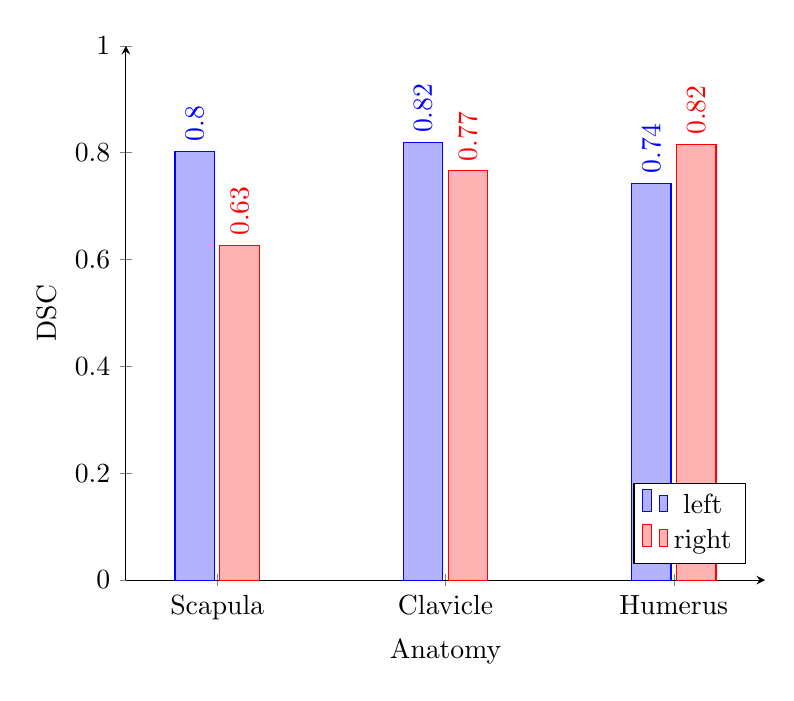
\begin{tikzpicture}
			\begin{axis}[
					width = 0.8\textwidth,
					xlabel = {Anatomy},
					ylabel = {DSC},
					bar width = 0.5cm,
					ymin = 0.00,
					ymax=1.00,
					ybar,
					axis y line = left,
					axis x line = bottom,
					xtick distance = 1,
					symbolic x coords = {Scapula, Clavicle, Humerus},
					legend pos = south east,
					nodes near coords,
					enlarge x limits = 0.2,
					every node near coord/.append style={anchor=west, rotate=90},
					compat=newest,]
				\addplot+ coordinates {(Scapula, 0.802739) (Clavicle, 0.818684) (Humerus, 0.74309) }; % left
				\addplot+ coordinates {(Scapula, 0.626175) (Clavicle, 0.765966) (Humerus, 0.815566) }; % right
				\legend{left, right};
			\end{axis}
		\end{tikzpicture}
		\caption{\acrshort{dc} results: Test person 1 (more is better)}\label{fig:dcs-tester1}
	\end{center}
\end{figure}
\begin{figure}[h!]
	\begin{subfigure}{0.49\linewidth}
		\centerline{
			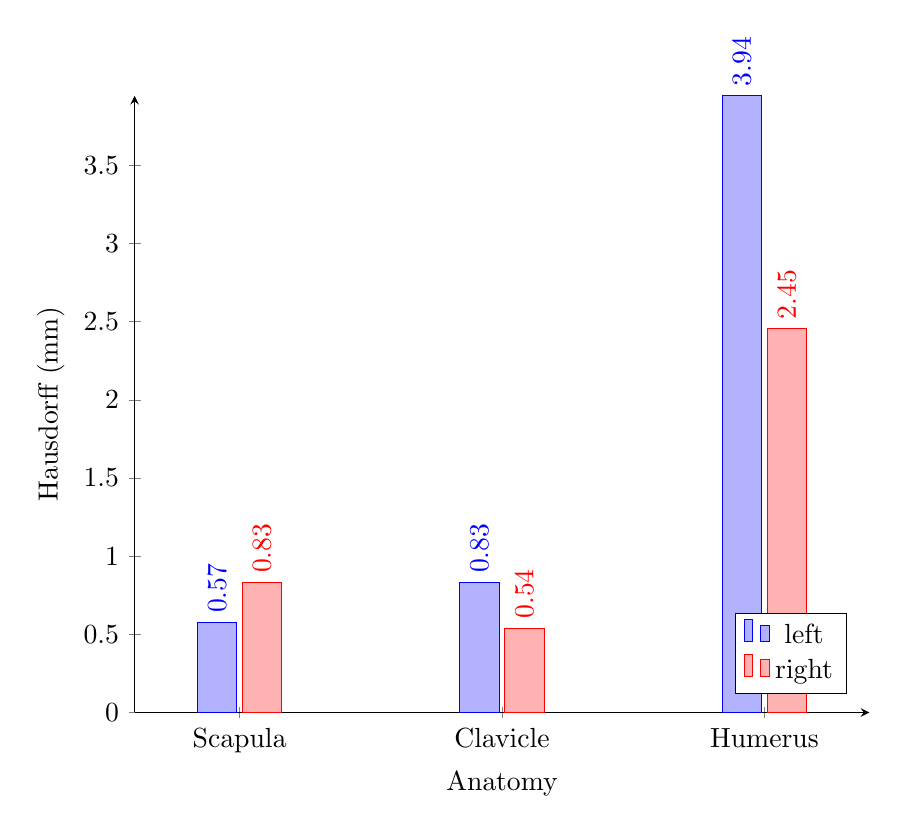
\begin{tikzpicture}
				\begin{axis}[
						width = 0.9\linewidth,
						xlabel = {Anatomy},
						ylabel = {Hausdorff (mm)},
						bar width = 0.5cm,
						ymin = 0.00, %ymax=1.00,
						ybar,
						axis y line = left,
						axis x line = bottom,
						xtick distance = 1,
						symbolic x coords = {Scapula, Clavicle, Humerus},
						legend pos = south east,
						nodes near coords,
						enlarge x limits = 0.2,
						every node near coord/.append style={anchor=west, rotate=90},
						compat=newest,]
					\addplot+ coordinates {(Scapula, 0.574456) (Clavicle, 0.830662) (Humerus, 3.94462) }; % left
					\addplot+ coordinates {(Scapula, 0.830662) (Clavicle, 0.538517) (Humerus, 2.45357) }; % right
					\legend{left, right};
				\end{axis}
			\end{tikzpicture}}
		\caption{\acrshort{hd} maximum results: Test person 1}\label{fig:t1-hd-max}
	\end{subfigure}
	\begin{subfigure}{0.49\linewidth}
		\centerline{
			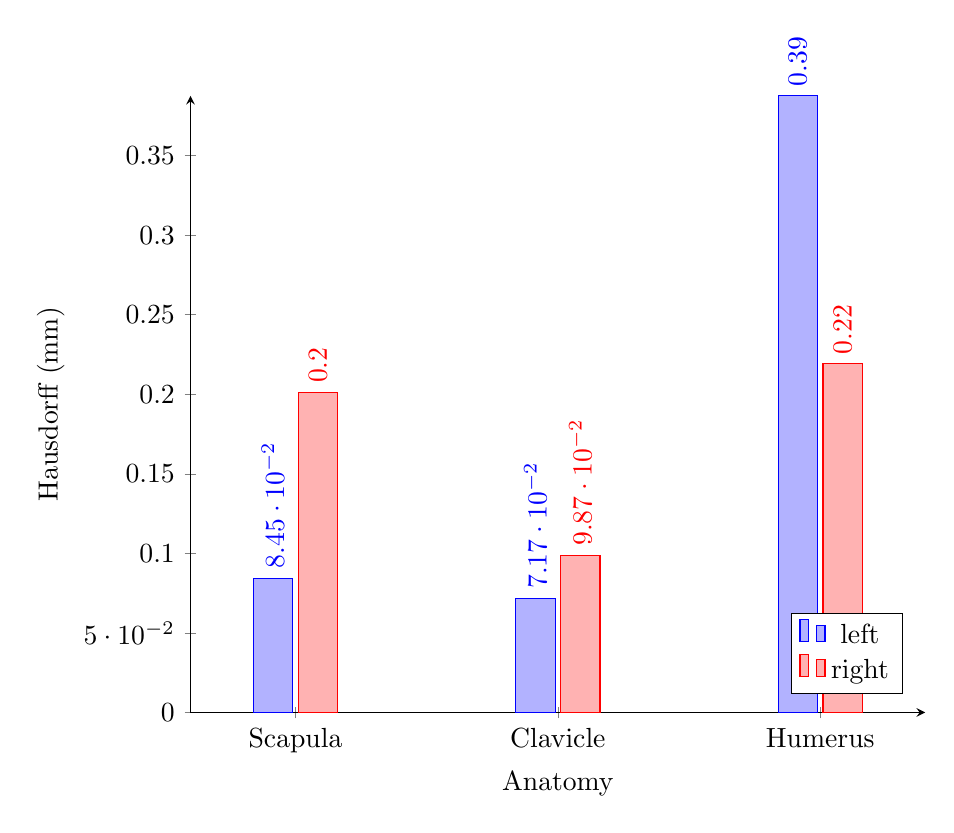
\begin{tikzpicture}
				\begin{axis}[
						width = 0.9\linewidth,
						xlabel = {Anatomy},
						ylabel = {Hausdorff (mm)},
						bar width = 0.5cm,
						ymin = 0.00,
						%ymax=1.00,
						ybar,
						axis y line = left,
						axis x line = bottom,
						xtick distance = 1,
						symbolic x coords = {Scapula, Clavicle, Humerus},
						legend pos = south east,
						nodes near coords,
						enlarge x limits = 0.2,
						every node near coord/.append style={anchor=west, rotate=90},
						compat=newest,]
					\addplot+ coordinates {(Scapula, 0.0844668) (Clavicle, 0.0716756) (Humerus, 0.387502) }; % left
					\addplot+ coordinates {(Scapula, 0.201003) (Clavicle, 0.0986822) (Humerus, 0.21904) }; % right
					\legend{left, right};
				\end{axis}
			\end{tikzpicture}}
		\caption{\acrshort{hd} average: Test person 1}\label{fig:t1-hd-avg}
	\end{subfigure}
	\caption{\acrfull{hd} results: Test person 1 (less is better)}\label{fig:hd-tester1}
\end{figure}
\noindent
\Cref{fig:dcs-tester1} illustrates the segmentation comparison results via the \acrfull{dc} for test participant 1.
The \acrshort{dc}-based segmentation overlap demonstrates a decline in accuracy for the scapula ($−0.17$) and clavicle ($−0.05$), while exhibiting an uptick for the humerus ($+0.08$).
\Cref{fig:hd-tester1} illustrates the segmentation comparison results via the \acrfull{hd} for test person 1.
Whereby \cref{fig:t1-hd-max} displays the maximum distance in millimeters (mm) while, \cref{fig:t1-hd-avg} displays the average distance in millimeters.
As can be seen, in \cref{fig:t1-hd-avg}, the segmentation of test person 1 on average was further from the ground truth in case of the scapula ($+0.1155 mm$) and clavicle ($+0.027 mm$).
With regard to the humerus, the segmentation was found to be in closer alignment with the ground truth, exhibiting a distance of ($−0.17mm$).


\section{Test person 2}\label{s:result-2}
\begin{figure}[h!]
	\begin{center}
		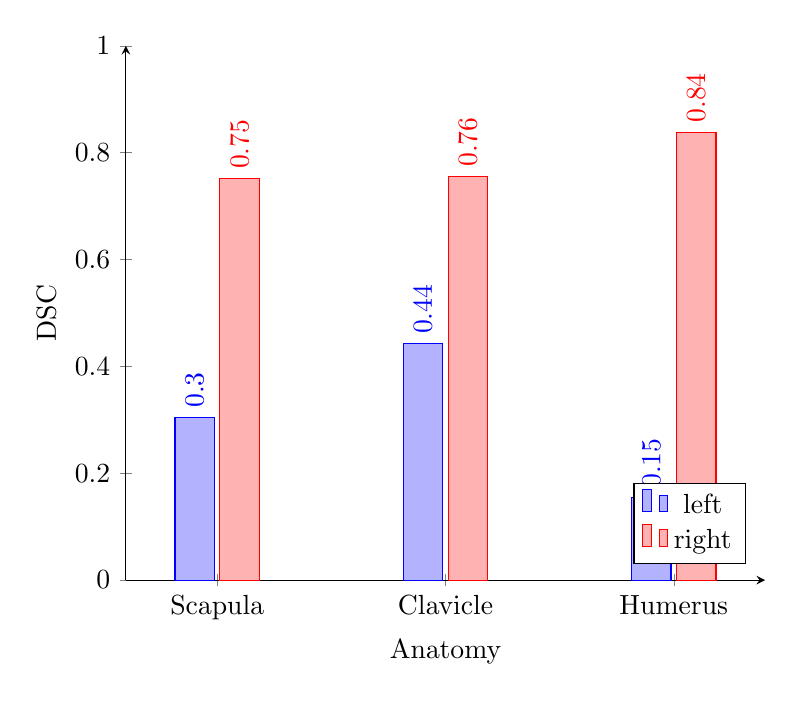
\begin{tikzpicture}
			\begin{axis}[
					width = 0.8\textwidth,
					xlabel = {Anatomy},
					ylabel = {DSC},
					bar width = 0.5cm,
					ymin = 0.00,
					ymax=1.00,
					ybar,
					axis y line = left,
					axis x line = bottom,
					xtick distance = 1,
					symbolic x coords = {Scapula, Clavicle, Humerus},
					legend pos = south east,
					nodes near coords,
					enlarge x limits = 0.2,
					every node near coord/.append style={anchor=west, rotate=90},
					compat=newest,]
				\addplot+ coordinates {(Scapula, 0.3043) (Clavicle, 0.442442) (Humerus, 0.154587) }; % left
				\addplot+ coordinates {(Scapula, 0.751427) (Clavicle, 0.755405) (Humerus, 0.838217) }; % right
				\legend{left, right};
			\end{axis}
		\end{tikzpicture}
		\caption{\acrshort{dc} results: Test person 2 (more is better)}\label{fig:dcs-tester2}
	\end{center}
\end{figure}
\begin{figure}[h!]
	\begin{subfigure}{0.49\linewidth}
		\centerline{
			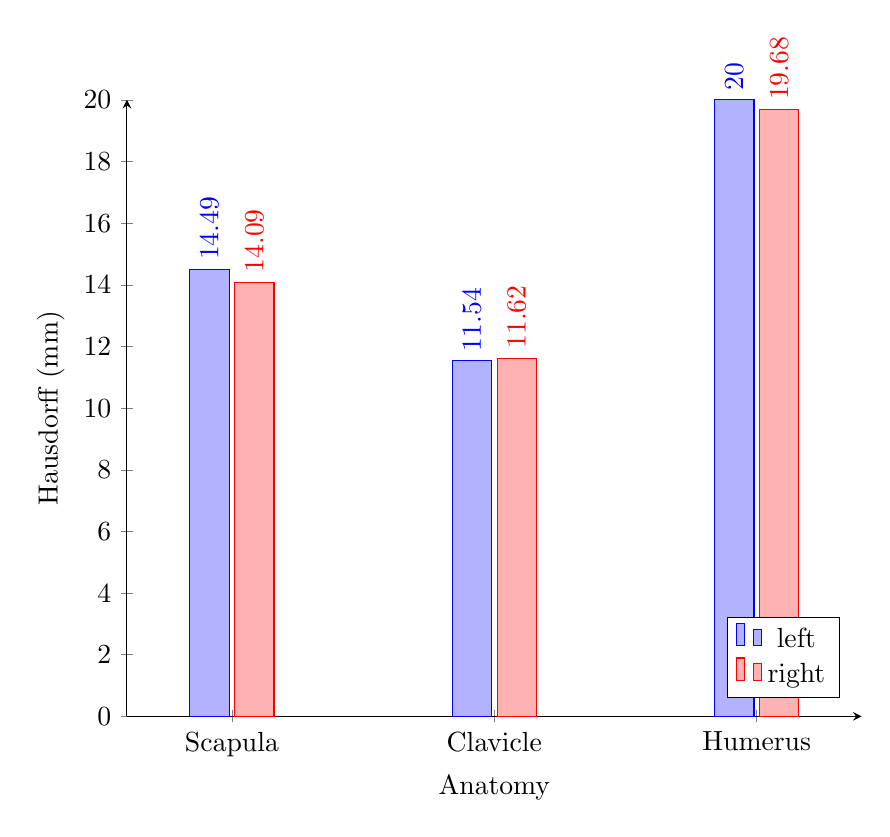
\begin{tikzpicture}
				\begin{axis}[
						width = 0.9\linewidth,
						xlabel = {Anatomy},
						ylabel = {Hausdorff (mm)},
						bar width = 0.5cm,
						ymin = 0.00, %ymax=1.00,
						ybar,
						axis y line = left,
						axis x line = bottom,
						xtick distance = 1,
						symbolic x coords = {Scapula, Clavicle, Humerus},
						legend pos = south east,
						nodes near coords,
						enlarge x limits = 0.2,
						every node near coord/.append style={anchor=west, rotate=90},
						compat=newest,]
					\addplot+ coordinates {(Scapula, 14.4948) (Clavicle, 11.5369) (Humerus, 20.004) }; % left
					\addplot+ coordinates {(Scapula, 14.0901) (Clavicle, 11.6224) (Humerus, 19.6827) }; % right
					\legend{left, right};
				\end{axis}
			\end{tikzpicture}}
		\caption{\acrshort{hd} maximum results: Test person 2}\label{fig:t2-hd-max}
	\end{subfigure}
	\begin{subfigure}{0.49\linewidth}
		\centerline{
			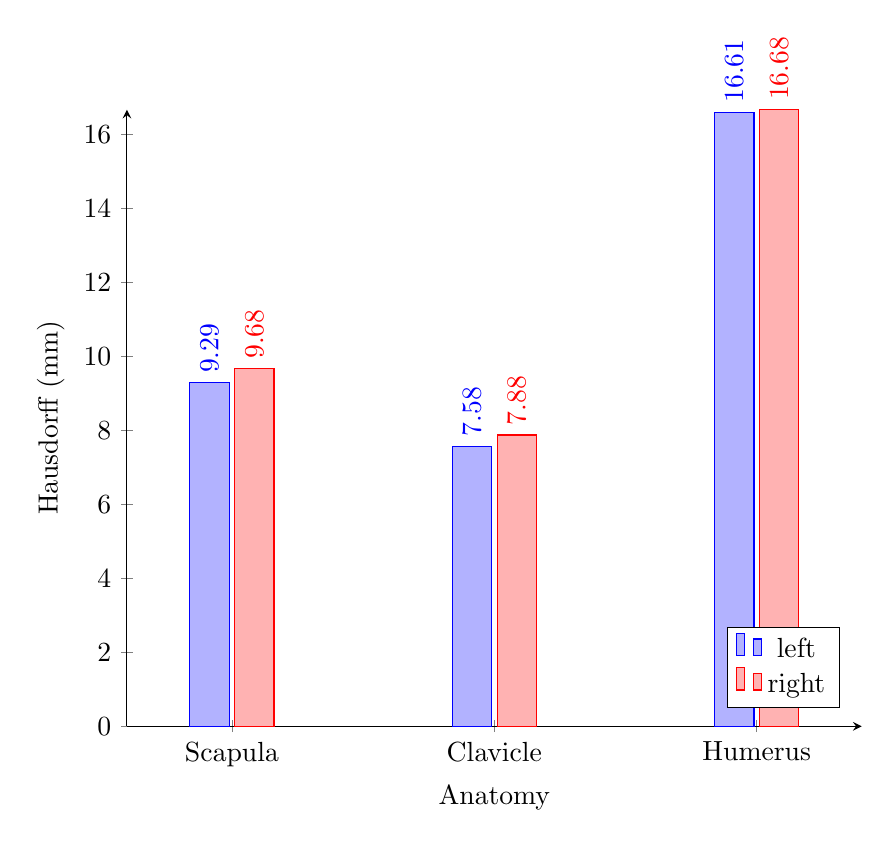
\begin{tikzpicture}
				\begin{axis}[
						width = 0.9\linewidth,
						xlabel = {Anatomy},
						ylabel = {Hausdorff (mm)},
						bar width = 0.5cm,
						ymin = 0.00,
						%ymax=1.00,
						ybar,
						axis y line = left,
						axis x line = bottom,
						xtick distance = 1,
						symbolic x coords = {Scapula, Clavicle, Humerus},
						legend pos = south east,
						nodes near coords,
						enlarge x limits = 0.2,
						every node near coord/.append style={anchor=west, rotate=90},
						compat=newest,
					]
					\addplot+ coordinates {(Scapula, 9.2935) (Clavicle, 7.5785) (Humerus, 16.6058) }; % left
					\addplot+ coordinates {(Scapula, 9.67503) (Clavicle, 7.87861) (Humerus, 16.6751) }; % right
					\legend{left, right};
				\end{axis}
			\end{tikzpicture}}
		\caption{\acrshort{hd} average: Test person 2}\label{fig:t2-hd-avg}
	\end{subfigure}
	\caption{\acrfull{hd} results: Test person 2 (less is better)}\label{fig:hd-tester2}
\end{figure}
\noindent
\Cref{fig:dcs-tester2} depicts the segmentation comparison results via the \acrfull{dc} for test person 2.
The segmentation overlap according to the \acrshort{dc} shows an increase in segmentation accuracy for all segmented anatomical structures: scapula ($+0.45$), clavicle ($+0.32$) and humerus ($+0.69$).
\Cref{fig:hd-tester2} depicts the segmentation comparison results via the \acrfull{hd} for test person 2.
Whereby \cref{fig:t2-hd-max} displays the maximum distance in millimeters (mm) and \cref{fig:t2-hd-avg} displays the average distance in millimeters.
As can be seen, in \cref{fig:t2-hd-avg}, the segmentation of test person 2 on average was slightly further from the ground truth for all segmented anatomical structures: scapula ($+0.39 mm$), clavicle ($+0.3 mm$) and humerus ($+0.07 mm$).


\section{Test person 3}\label{s:result-3}
\begin{figure}[h!]
	\begin{center}
		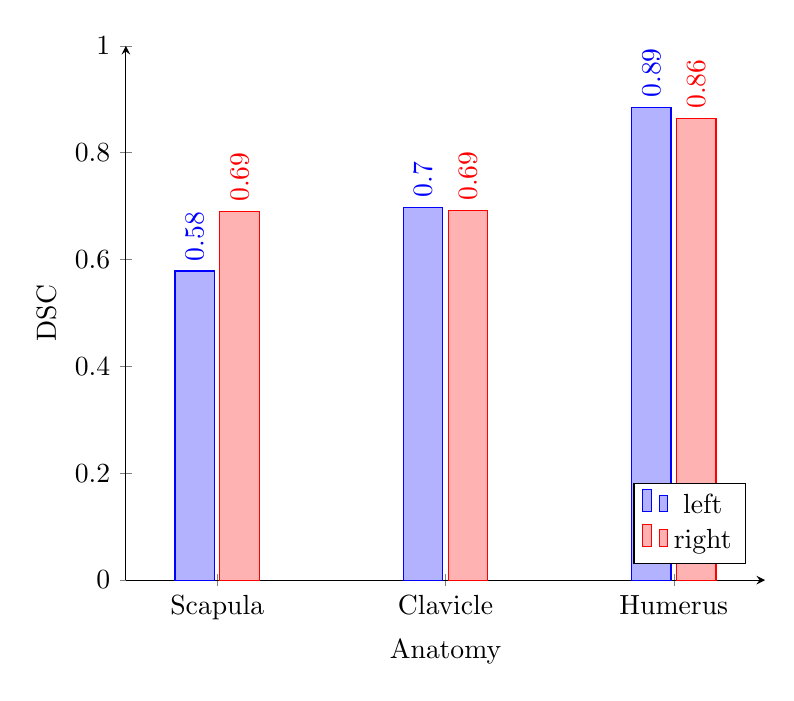
\begin{tikzpicture}
			\begin{axis}[
					width = 0.8\textwidth,
					xlabel = {Anatomy},
					ylabel = {DSC},
					bar width = 0.5cm,
					ymin = 0.00,
					ymax=1.00,
					ybar,
					axis y line = left,
					axis x line = bottom,
					xtick distance = 1,
					symbolic x coords = {Scapula, Clavicle, Humerus},
					legend pos = south east,
					nodes near coords,
					enlarge x limits = 0.2,
					every node near coord/.append style={anchor=west, rotate=90},
					compat=newest,]
				\addplot+ coordinates {(Scapula, 0.578573) (Clavicle, 0.6981) (Humerus, 0.885087) }; % left
				\addplot+ coordinates {(Scapula, 0.689855) (Clavicle, 0.691658) (Humerus, 0.864106) }; % right
				\legend{left, right};
			\end{axis}
		\end{tikzpicture}
		\caption{\acrshort{dc} results: Test person 3 (more is better)}\label{fig:dcs-tester3}
	\end{center}
\end{figure}
\begin{figure}[h!]
	\begin{subfigure}{0.49\linewidth}
		\centerline{
			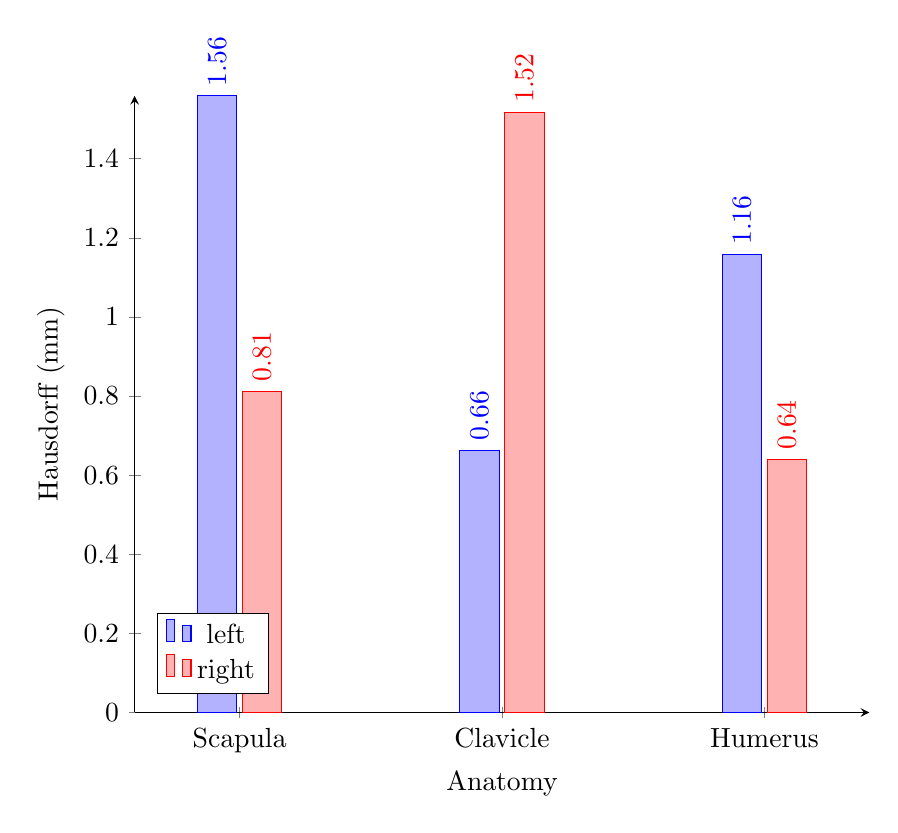
\begin{tikzpicture}
				\begin{axis}[
						width = 0.9\linewidth,
						xlabel = {Anatomy},
						ylabel = {Hausdorff (mm)},
						bar width = 0.5cm,
						ymin = 0.00, %ymax=1.00,
						ybar,
						axis y line = left,
						axis x line = bottom,
						xtick distance = 1,
						symbolic x coords = {Scapula, Clavicle, Humerus},
						legend pos = south west,
						nodes near coords,
						enlarge x limits = 0.2,
						every node near coord/.append style={anchor=west, rotate=90},
						compat=newest,]
					\addplot+ coordinates {(Scapula, 1.55885) (Clavicle, 0.663325) (Humerus, 1.15758) }; % left
					\addplot+ coordinates {(Scapula, 0.812404) (Clavicle, 1.51658) (Humerus, 0.640312) }; % right
					\legend{left, right};
				\end{axis}
			\end{tikzpicture}}
		\caption{\acrshort{hd} maximum results: Test person 3}\label{fig:t3-hd-max}
	\end{subfigure}
	\begin{subfigure}{0.49\linewidth}
		\centerline{
			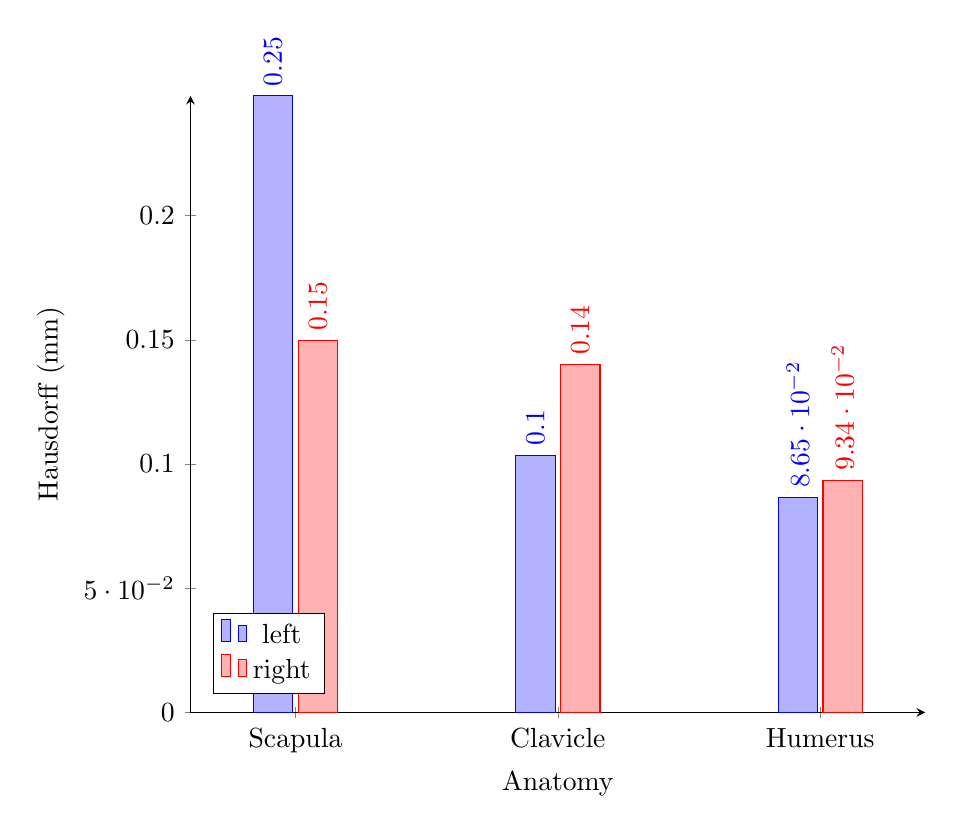
\begin{tikzpicture}
				\begin{axis}[
						width = 0.9\linewidth,
						xlabel = {Anatomy},
						ylabel = {Hausdorff (mm)},
						bar width = 0.5cm,
						ymin = 0.00,
						%ymax=1.00,
						ybar,
						axis y line = left,
						axis x line = bottom,
						xtick distance = 1,
						symbolic x coords = {Scapula, Clavicle, Humerus},
						legend pos = south west,
						nodes near coords,
						enlarge x limits = 0.2,
						every node near coord/.append style={anchor=west, rotate=90},
						compat=newest,]
					\addplot+ coordinates {(Scapula, 0.248237) (Clavicle, 0.103545) (Humerus, 0.0864548) }; % left
					\addplot+ coordinates {(Scapula, 0.149758) (Clavicle, 0.140087) (Humerus, 0.0934432) }; % right
					\legend{left, right};
				\end{axis}
			\end{tikzpicture}}
		\caption{\acrshort{hd} average: Test person 3}\label{fig:t3-hd-avg}
	\end{subfigure}
	\caption{\acrfull{hd} results: Test person 3 (less is better)}\label{fig:hd-tester3}
\end{figure}
\noindent
\Cref{fig:dcs-tester3} serves as a depiction of the segmentation results compared with the \acrfull{dc} for test participant 3.
The segmentation overlap shows an uptick in segmentation accuracy for the scapula ($+0.11$) and a decrease for the clavicle ($-0.01$) as well as the humerus ($-0.03$).
\Cref{fig:hd-tester3} illustrates the segmentation results for test participant 3 compared via the \acrfull{hd}.
Whereby \cref{fig:t3-hd-max} displays the maximum distance in millimeters (mm) and \cref{fig:t3-hd-avg} displays the average distance in millimeters.
As can be seen, in \cref{fig:t3-hd-avg}, the segmentation of test person 3 on average was actually closer to the ground truth for the scapula ($-0.1 mm$) and further from it for clavicle ($+0.04 mm$) and humerus ($+0.0069 mm$).


\section{Test person 4}\label{s:result-4}
\begin{figure}[h!]
	\begin{center}
		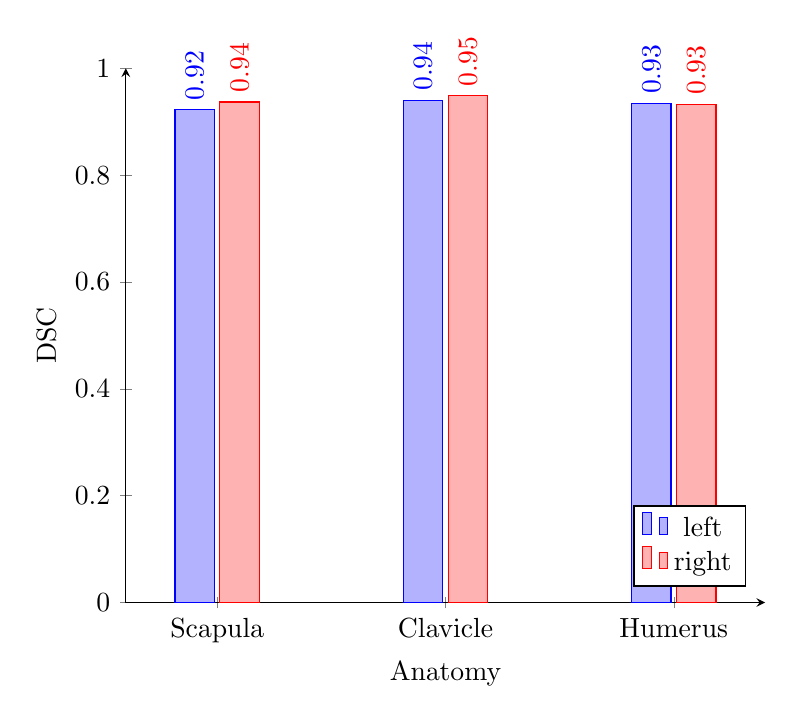
\begin{tikzpicture}
			\begin{axis}[
					width = 0.8\textwidth,
					xlabel = {Anatomy},
					ylabel = {DSC},
					bar width = 0.5cm,
					ymin = 0.00,
					ymax=1.00,
					ybar,
					axis y line = left,
					axis x line = bottom,
					xtick distance = 1,
					symbolic x coords = {Scapula, Clavicle, Humerus},
					legend pos = south east,
					nodes near coords,
					enlarge x limits = 0.2,
					every node near coord/.append style={anchor=west, rotate=90},
					compat=newest,]
				\addplot+ coordinates {(Scapula, 0.922192) (Clavicle, 0.939727) (Humerus, 0.933602) }; % left
				\addplot+ coordinates {(Scapula, 0.936915) (Clavicle, 0.94835) (Humerus, 0.932487) }; % right
				\legend{left, right};
			\end{axis}
		\end{tikzpicture}
		\caption{\acrshort{dc} results: Test person 4 (more is better)}\label{fig:dcs-tester4}
	\end{center}
\end{figure}
\begin{figure}[h!]
	\begin{subfigure}{0.49\linewidth}
		\centerline{
			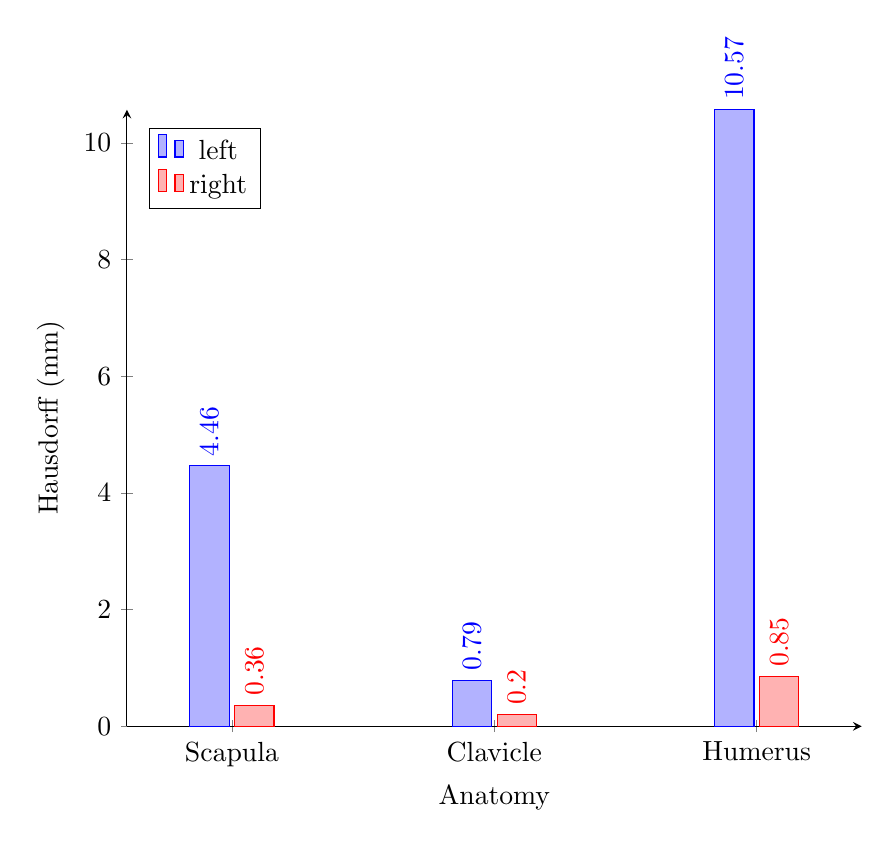
\begin{tikzpicture}
				\begin{axis}[
						width = 0.9\linewidth,
						xlabel = {Anatomy},
						ylabel = {Hausdorff (mm)},
						bar width = 0.5cm,
						ymin = 0.00, %ymax=1.00,
						ybar,
						axis y line = left,
						axis x line = bottom,
						xtick distance = 1,
						symbolic x coords = {Scapula, Clavicle, Humerus},
						legend pos = north west,
						nodes near coords,
						enlarge x limits = 0.2,
						every node near coord/.append style={anchor=west, rotate=90},
						compat=newest,]
					\addplot+ coordinates {(Scapula, 4.4643) (Clavicle, 0.787401) (Humerus, 10.5669) }; % left
					\addplot+ coordinates {(Scapula, 0.360555) (Clavicle, 0.2) (Humerus, 0.8544) }; % right
					\legend{left, right};
				\end{axis}
			\end{tikzpicture}}
		\caption{\acrshort{hd} maximum results: Test person 4}\label{fig:t4-hd-max}
	\end{subfigure}
	\begin{subfigure}{0.49\linewidth}
		\centerline{
			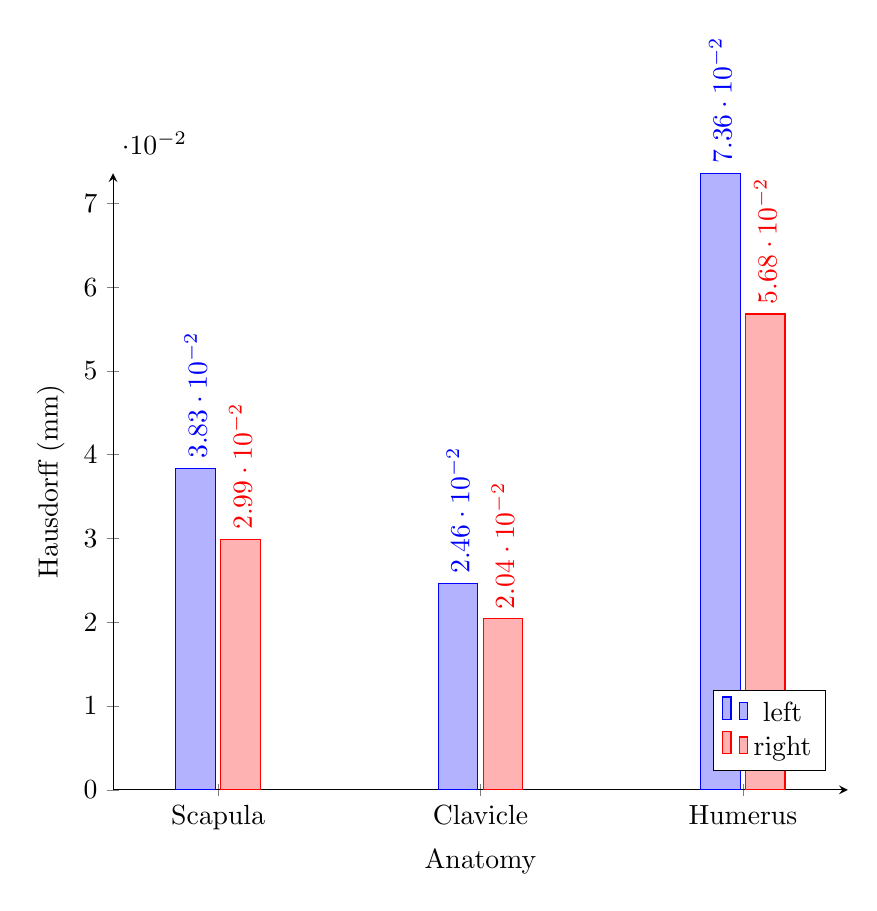
\begin{tikzpicture}
				\begin{axis}[
						width = 0.9\linewidth,
						xlabel = {Anatomy},
						ylabel = {Hausdorff (mm)},
						bar width = 0.5cm,
						ymin = 0.00,
						%ymax=1.00,
						ybar,
						axis y line = left,
						axis x line = bottom,
						xtick distance = 1,
						symbolic x coords = {Scapula, Clavicle, Humerus},
						legend pos = south east,
						nodes near coords,
						enlarge x limits = 0.2,
						every node near coord/.append style={anchor=west, rotate=90},
						compat=newest,]
					\addplot+ coordinates {(Scapula, 0.0383409) (Clavicle, 0.0246443) (Humerus, 0.0735903) }; % left
					\addplot+ coordinates {(Scapula, 0.0298934) (Clavicle, 0.0204125) (Humerus, 0.0567954) }; % right
					\legend{left, right};
				\end{axis}
			\end{tikzpicture}}
		\caption{\acrshort{hd} average: Test person 4}\label{fig:t4-hd-avg}
	\end{subfigure}
	\caption{\acrfull{hd} results: Test person 4 (less is better)}\label{fig:hd-tester4}
\end{figure}
\noindent
The segmentation comparison results using the \acrfull{dc} for test person 4 are shown in \cref{fig:dcs-tester4}.
Two of the three segmentations, scapula ($+0.02$) and clavicle ($+0.01$), show an improvement in segmentation accuracy.
Whereas, the humerus exhibits no change in segmentation overlap as determined by the \acrshort{dc}.
The segmentation comparison results using the Hausdorff distance (HD) for test person 4 are shown in \cref{fig:hd-tester4}.
Whereas \cref{fig:t4-hd-max} shows the average distance in millimeters, Figure 39a shows the greatest distance in millimeters (mm).
As shown in \cref{fig:t4-hd-avg}, test person 2's segmentation was, on average, closer to the ground truth in all cases: scapula ($-0.0084 mm$), clavicle ($-0.0042 mm$) and humerus ($-0.0168 mm$).


\section{Test person 5}\label{s:result-5}
\begin{figure}[h!]
	\begin{center}
		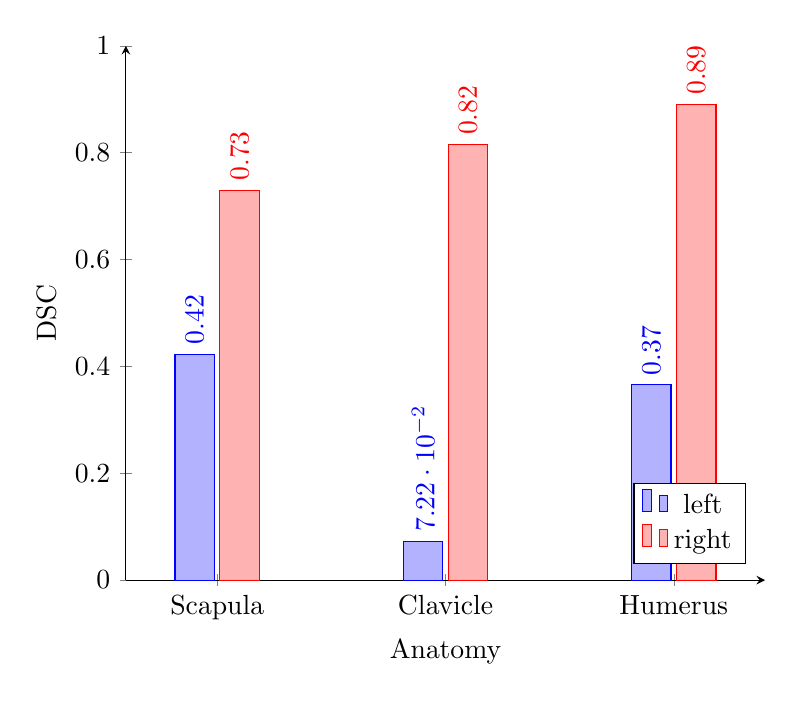
\begin{tikzpicture}
			\begin{axis}[
					width = 0.8\textwidth,
					xlabel = {Anatomy},
					ylabel = {DSC},
					bar width = 0.5cm,
					ymin = 0.00,
					ymax=1.00,
					ybar,
					axis y line = left,
					axis x line = bottom,
					xtick distance = 1,
					symbolic x coords = {Scapula, Clavicle, Humerus},
					legend pos = south east,
					nodes near coords,
					enlarge x limits = 0.2,
					every node near coord/.append style={anchor=west, rotate=90},
					compat=newest,]
				\addplot+ coordinates {(Scapula, 0.422959) (Clavicle, 0.0721612) (Humerus, 0.365373) }; % left
				\addplot+ coordinates {(Scapula, 0.729698) (Clavicle, 0.815007) (Humerus, 0.890025) }; % right
				\legend{left, right};
			\end{axis}
		\end{tikzpicture}
		\caption{\acrshort{dc} results: Test person 5 (more is better)}\label{fig:dcs-tester5}
	\end{center}
\end{figure}
\begin{figure}[h!]
	\begin{subfigure}{0.49\linewidth}
		\centerline{
			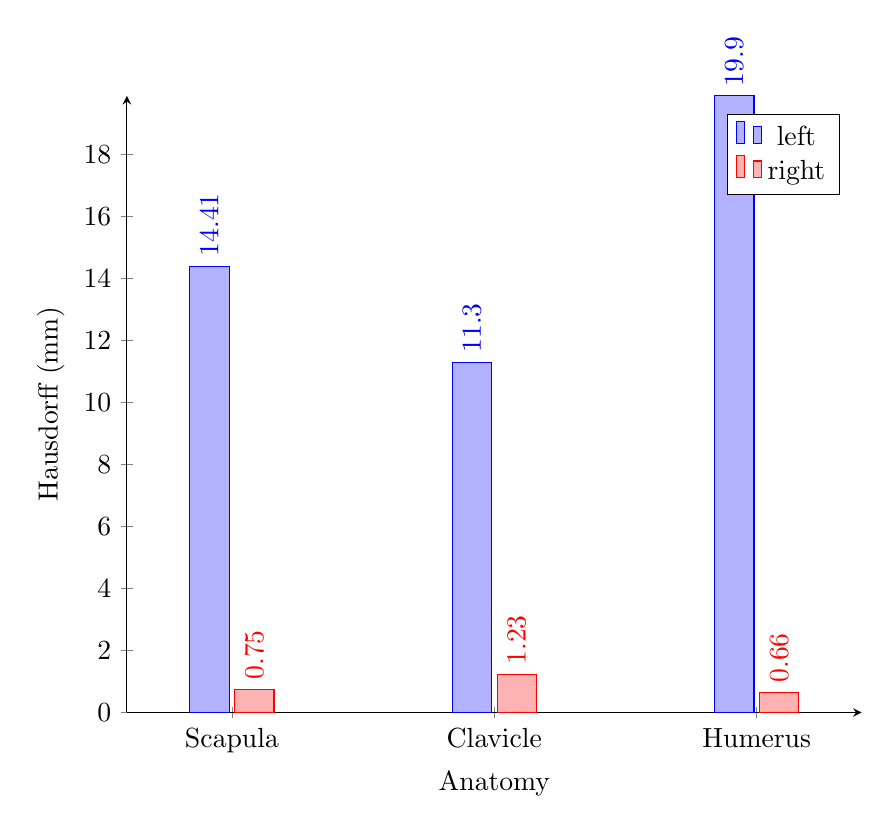
\begin{tikzpicture}
				\begin{axis}[
						width = 0.9\linewidth,
						xlabel = {Anatomy},
						ylabel = {Hausdorff (mm)},
						bar width = 0.5cm,
						ymin = 0.00, %ymax=1.00,
						ybar,
						axis y line = left,
						axis x line = bottom,
						xtick distance = 1,
						symbolic x coords = {Scapula, Clavicle, Humerus},
						legend pos = north east,
						nodes near coords,
						enlarge x limits = 0.2,
						every node near coord/.append style={anchor=west, rotate=90},
						compat=newest,]
					\addplot+ coordinates {(Scapula, 14.4066) (Clavicle, 11.2987) (Humerus, 19.9) }; % left
					\addplot+ coordinates {(Scapula, 0.748331) (Clavicle, 1.23288) (Humerus, 0.655744) }; % right
					\legend{left, right};
				\end{axis}
			\end{tikzpicture}}
		\caption{\acrshort{hd} maximum results: Test person 5}\label{fig:t5-hd-max}
	\end{subfigure}
	\begin{subfigure}{0.49\linewidth}
		\centerline{
			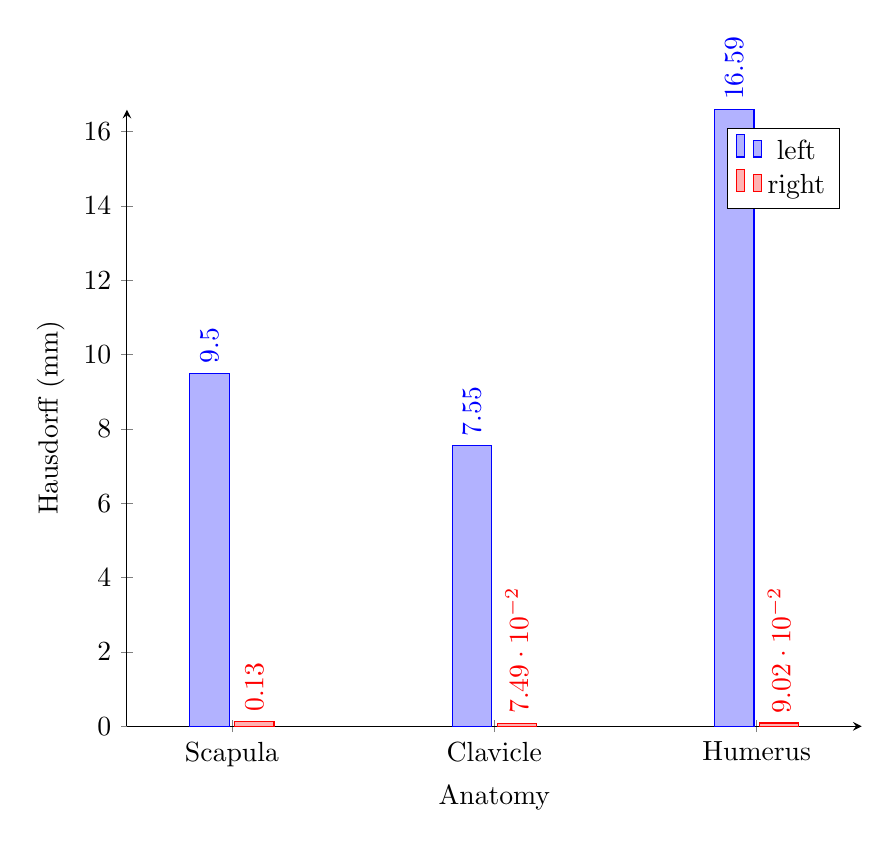
\begin{tikzpicture}
				\begin{axis}[
						width = 0.9\linewidth,
						xlabel = {Anatomy},
						ylabel = {Hausdorff (mm)},
						bar width = 0.5cm,
						ymin = 0.00,%ymax=1.00,
						ybar,
						axis y line = left,
						axis x line = bottom,
						xtick distance = 1,
						symbolic x coords = {Scapula, Clavicle, Humerus},
						legend pos = north east,
						nodes near coords,
						enlarge x limits = 0.2,
						every node near coord/.append style={anchor=west, rotate=90},
						compat=newest,]
					\addplot+ coordinates {(Scapula, 9.49633) (Clavicle, 7.54572) (Humerus, 16.5861) }; % left
					\addplot+ coordinates {(Scapula, 0.130622) (Clavicle, 0.0749329) (Humerus, 0.0901881) }; % right
					\legend{left, right};
				\end{axis}
			\end{tikzpicture}}
		\caption{\acrshort{hd} average: Test person 5}\label{fig:t5-hd-avg}
	\end{subfigure}
	\caption{\acrfull{hd} results: Test person 5 (less is better)}\label{fig:hd-tester5}
\end{figure}
\noindent
\Cref{fig:dcs-tester5} illustrates the segmentation comparison results using the \acrfull{dc} for test person 5.
The \acrshort{dc}'s segmentation overlap indicates that all segmented anatomical structures—the scapula ($+0.31$), clavicle ($+0.7478$), and humerus ($+0.52$)—have improved segmentation accuracy.
The segmentation comparison results for test participant 5 using the \acrfull{hd} are shown in \cref{fig:hd-tester5}.
Whereas \cref{fig:t5-hd-max} displays the maximum distance in millimeters (mm) and \cref{fig:t5-hd-avg} displays the average distance in millimeters.
\Cref{fig:t5-hd-avg} shows that, on average, test person 5's segmentation of the scapula ($−9.37mm$), clavicle ($−7.4751mm$), and humerus ($−16.4959mm$) was closer to the ground truth in every instance.


\section{Test person 6}\label{s:result-6}
\begin{figure}[h!]
	\begin{center}
		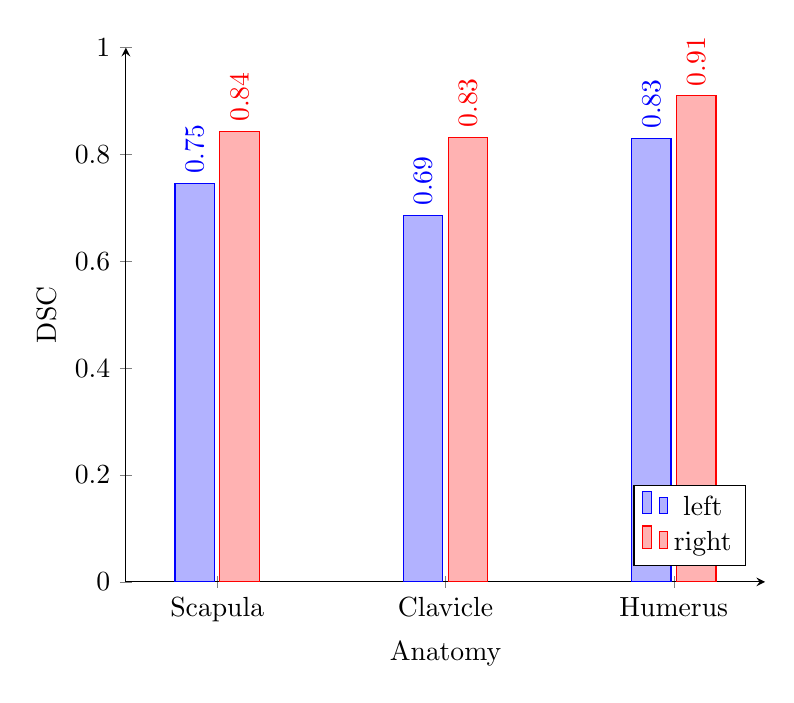
\begin{tikzpicture}
			\begin{axis}[
					width = 0.8\textwidth,
					xlabel = {Anatomy},
					ylabel = {DSC},
					bar width = 0.5cm,
					ymin = 0.00,
					ymax=1.00,
					ybar,
					axis y line = left,
					axis x line = bottom,
					xtick distance = 1,
					symbolic x coords = {Scapula, Clavicle, Humerus},
					legend pos = south east,
					nodes near coords,
					enlarge x limits = 0.2,
					every node near coord/.append style={anchor=west, rotate=90},
					compat=newest,]
				\addplot+ coordinates {(Scapula, 0.745496) (Clavicle, 0.685963) (Humerus, 0.8301) }; % left
				\addplot+ coordinates {(Scapula, 0.843293) (Clavicle, 0.832382) (Humerus, 0.90979) }; % right
				\legend{left, right};
			\end{axis}
		\end{tikzpicture}
		\caption{\acrshort{dc} results: Test person 6 (more is better)}\label{fig:dcs-tester6}
	\end{center}
\end{figure}
\begin{figure}[h!]
	\begin{subfigure}{0.49\linewidth}
		\centerline{
			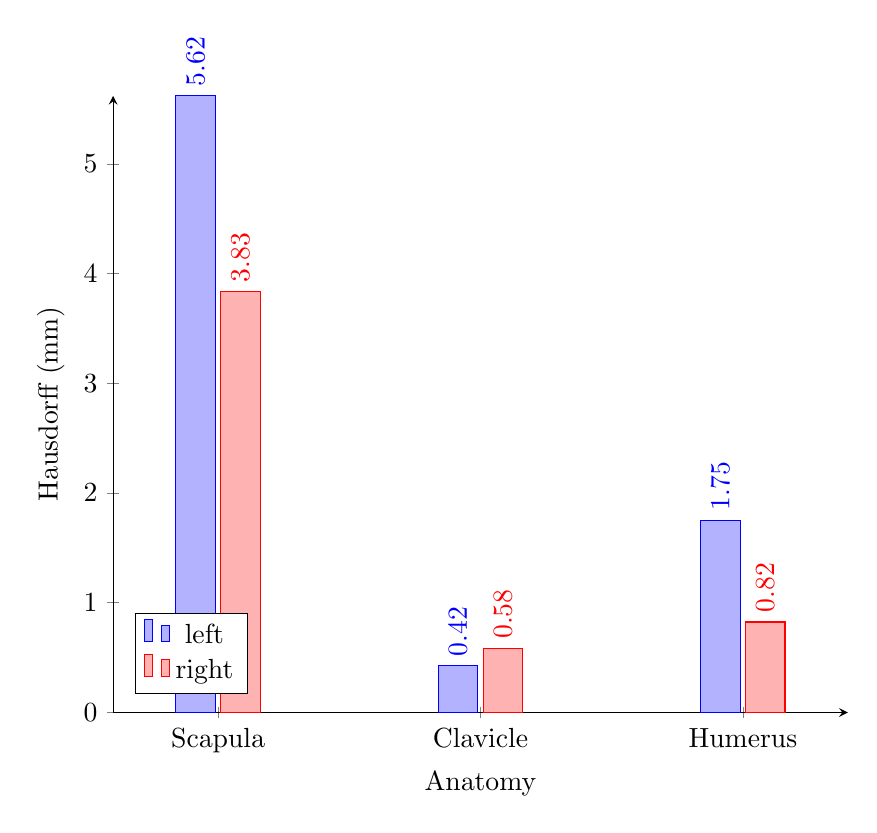
\begin{tikzpicture}
				\begin{axis}[
						width = 0.9\linewidth,
						xlabel = {Anatomy},
						ylabel = {Hausdorff (mm)},
						bar width = 0.5cm,
						ymin = 0.00,%ymax=1.00,
						ybar,
						axis y line = left,
						axis x line = bottom,
						xtick distance = 1,
						symbolic x coords = {Scapula, Clavicle, Humerus},
						legend pos = south west,
						nodes near coords,
						enlarge x limits = 0.2,
						every node near coord/.append style={anchor=west, rotate=90},
						compat=newest,]
					\addplot+ coordinates {(Scapula, 5.61961) (Clavicle, 0.424264) (Humerus, 1.74929) }; % left
					\addplot+ coordinates {(Scapula, 3.83275) (Clavicle, 0.583095) (Humerus, 0.824621) }; % right
					\legend{left, right};
				\end{axis}
			\end{tikzpicture}}
		\caption{\acrshort{hd} maximum results: Test person 6}\label{fig:t6-hd-max}
	\end{subfigure}
	\begin{subfigure}{0.49\linewidth}
		\centerline{
			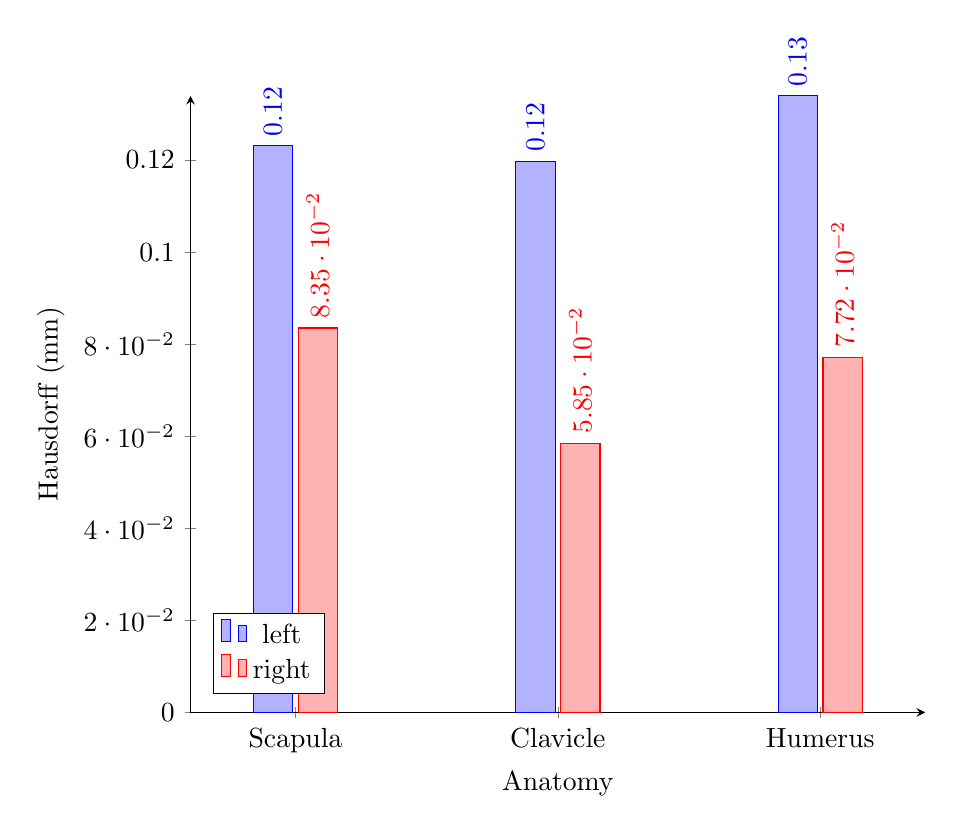
\begin{tikzpicture}
				\begin{axis}[
						width = 0.9\linewidth,
						xlabel = {Anatomy},
						ylabel = {Hausdorff (mm)},
						bar width = 0.5cm,
						ymin = 0.00,
						%ymax=1.00,
						ybar,
						axis y line = left,
						axis x line = bottom,
						xtick distance = 1,
						symbolic x coords = {Scapula, Clavicle, Humerus},
						legend pos = south west,
						nodes near coords,
						enlarge x limits = 0.2,
						every node near coord/.append style={anchor=west, rotate=90},
						compat=newest,]
					\addplot+ coordinates {(Scapula, 0.12307) (Clavicle, 0.119685) (Humerus, 0.133942) }; % left
					\addplot+ coordinates {(Scapula, 0.0835118) (Clavicle, 0.0584966) (Humerus, 0.077168) }; % right
					\legend{left, right};
				\end{axis}
			\end{tikzpicture}}
		\caption{\acrshort{hd} average: Test person 6}\label{fig:t6-hd-avg}
	\end{subfigure}
	\caption{\acrfull{hd} results: Test person 6 (less is better)}\label{fig:hd-tester6}
\end{figure}
\noindent
The segmentation comparison results using the \acrfull{dc} for test person 6 are shown in \cref{fig:dcs-tester6}.
The clavicle ($+0.14$), humerus ($+0.08$), and scapula ($+0.09$) all exhibit improved segmentation accuracy, according to the \acrshort{dc}'s segmentation overlap.
The segmentation comparison results using the \acrfull{hd} for test person 6 are shown in \cref{fig:hd-tester6}.
Whereas \cref{fig:t6-hd-avg} shows the average distance in millimeters, \cref{fig:t6-hd-max} shows the greatest distance in millimeters (mm).
Test person 6's segmentation, as shown in \cref{fig:t6-hd-avg}, was generally closer to the ground truth in all cases: scapula ($−0.0365mm$), clavicle ($−0.0615mm$), and humerus ($−0.0528mm$).



\section{Test person 7}\label{s:result-7}
\begin{figure}[h!]
	\begin{center}
		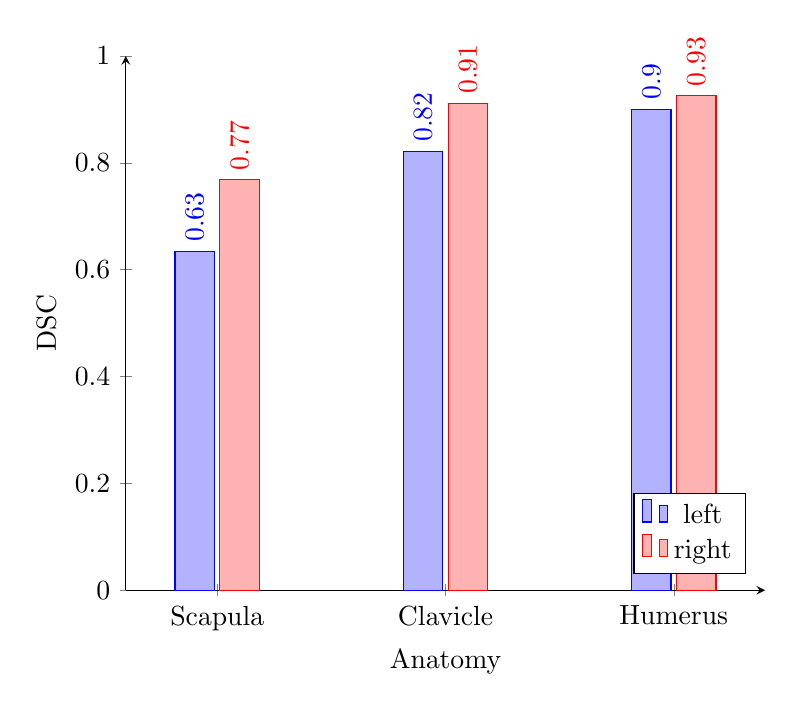
\begin{tikzpicture}
			\begin{axis}[
					width = 0.8\textwidth,
					xlabel = {Anatomy},
					ylabel = {DSC},
					bar width = 0.5cm,
					ymin = 0.00,
					ymax=1.00,
					ybar,
					axis y line = left,
					axis x line = bottom,
					xtick distance = 1,
					symbolic x coords = {Scapula, Clavicle, Humerus},
					legend pos = south east,
					nodes near coords,
					enlarge x limits = 0.2,
					every node near coord/.append style={anchor=west, rotate=90},
					compat=newest,]
				\addplot+ coordinates {(Scapula, 0.634313) (Clavicle, 0.821007) (Humerus, 0.900482) }; % left
				\addplot+ coordinates {(Scapula, 0.76807) (Clavicle, 0.911396) (Humerus, 0.925331) }; % right
				\legend{left, right};
			\end{axis}
		\end{tikzpicture}
		\caption{\acrshort{dc} results: Test person 7 (more is better)}\label{fig:dcs-tester7}
	\end{center}
\end{figure}
\begin{figure}[h!]
	\begin{subfigure}{0.49\linewidth}
		\centerline{
			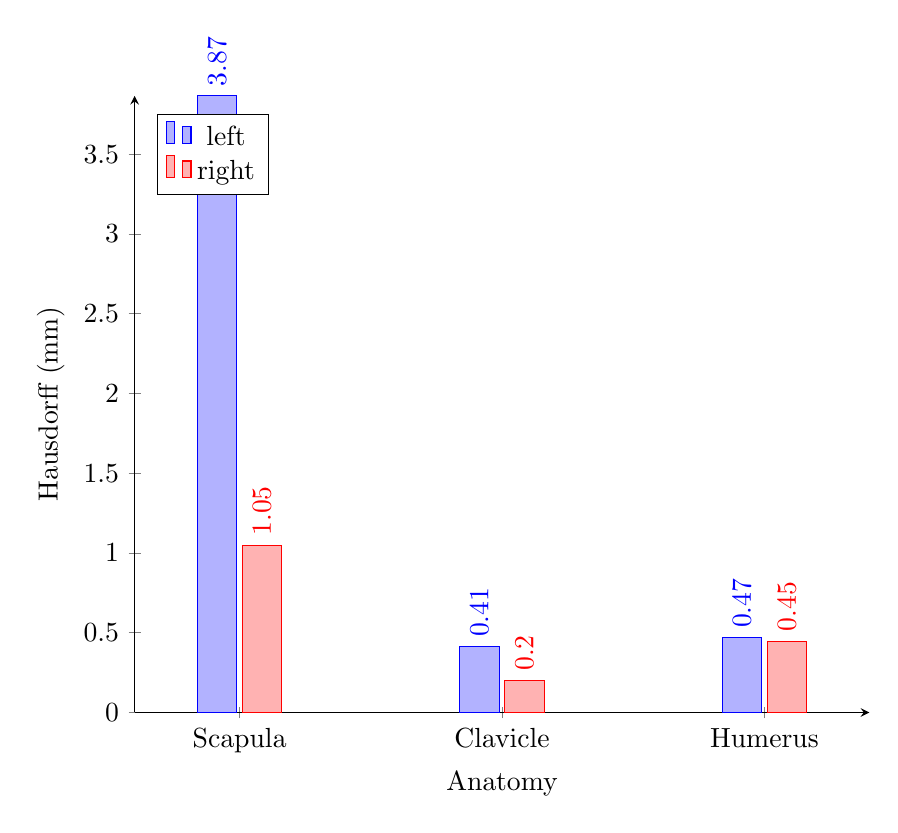
\begin{tikzpicture}
				\begin{axis}[
						width = 0.9\linewidth,
						xlabel = {Anatomy},
						ylabel = {Hausdorff (mm)},
						bar width = 0.5cm,
						ymin = 0.00,%ymax=1.00,
						ybar,
						axis y line = left,
						axis x line = bottom,
						xtick distance = 1,
						symbolic x coords = {Scapula, Clavicle, Humerus},
						legend pos = north west,
						nodes near coords,
						enlarge x limits = 0.2,
						every node near coord/.append style={anchor=west, rotate=90},
						compat=newest,]
					\addplot+ coordinates {(Scapula, 3.86523) (Clavicle, 0.412311) (Humerus, 0.469042) }; % left
					\addplot+ coordinates {(Scapula, 1.04881) (Clavicle, 0.2) (Humerus, 0.447214) }; % right
					\legend{left, right};
				\end{axis}
			\end{tikzpicture}}
		\caption{\acrshort{hd} maximum results: Test person 7}\label{fig:t7-hd-max}
	\end{subfigure}
	\begin{subfigure}{0.49\linewidth}
		\centerline{
			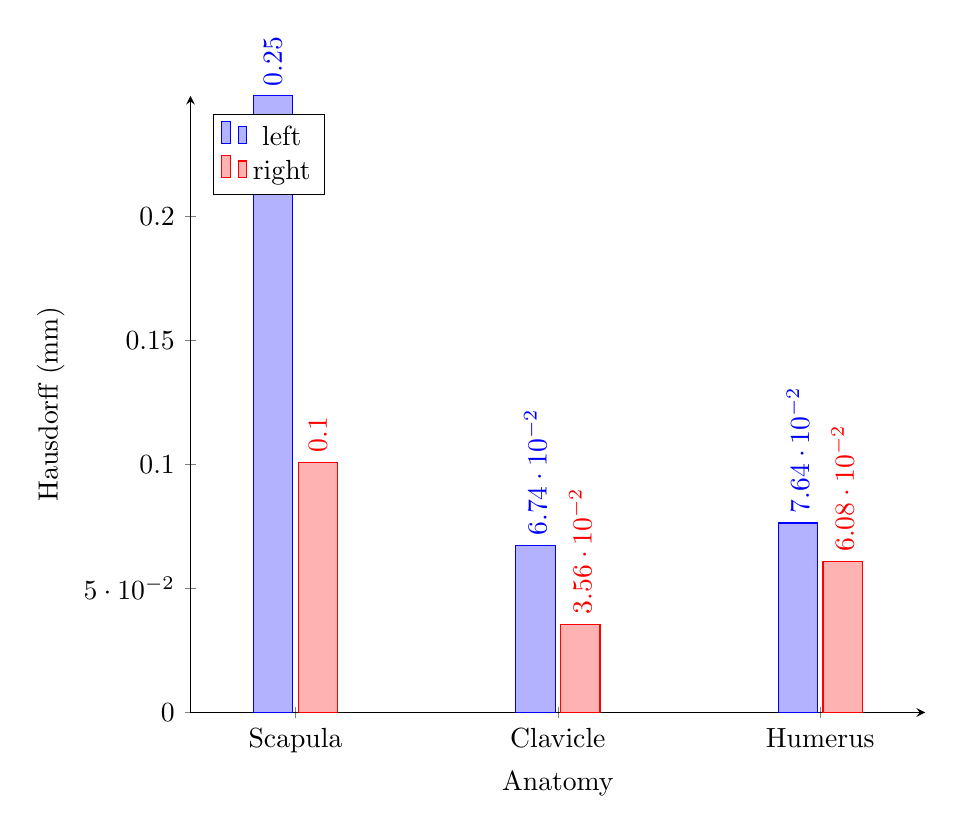
\begin{tikzpicture}
				\begin{axis}[
						width = 0.9\linewidth,
						xlabel = {Anatomy},
						ylabel = {Hausdorff (mm)},
						bar width = 0.5cm,
						ymin = 0.00,%ymax=1.00,
						ybar,
						axis y line = left,
						axis x line = bottom,
						xtick distance = 1,
						symbolic x coords = {Scapula, Clavicle, Humerus},
						legend pos = north west,
						nodes near coords,
						enlarge x limits = 0.2,
						every node near coord/.append style={anchor=west, rotate=90},
						compat=newest,]
					\addplot+ coordinates {(Scapula, 0.24856) (Clavicle, 0.0674237) (Humerus, 0.0763588) }; % left
					\addplot+ coordinates {(Scapula, 0.100908) (Clavicle, 0.0356212) (Humerus, 0.0608241) }; % right
					\legend{left, right};
				\end{axis}
			\end{tikzpicture}}
		\caption{\acrshort{hd} average: Test person 7}\label{fig:t7-hd-avg}
	\end{subfigure}
	\caption{\acrfull{hd} results: Test person 7 (less is better)}\label{fig:hd-tester7}
\end{figure}
\noindent
\Cref{fig:dcs-tester7} depicts the segmentation comparison results via the \acrfull{dc} for test person 7.
The segmentation overlap according to the \acrshort{dc} shows an increase in segmentation accuracy in all segmented anatomical structures: scapula ($+0.14$), clavicle ($+0.09$) and humerus ($+0.03$).
\Cref{fig:hd-tester7} depicts the segmentation comparison results via the \acrfull{hd} for test person 7.
Whereby \cref{fig:t7-hd-max} displays the maximum distance in millimeters (mm) and \cref{fig:t7-hd-avg} displays the average distance in millimeters.
As can be seen, in \cref{fig:t7-hd-avg}, the segmentation of test person 7 on average was closer to the ground truth in all cases: scapula ($-0.15 mm$), clavicle ($-0.0318 mm$) and humerus ($-0.0156 mm$).

